\documentclass[border=10pt]{standalone}
\usepackage{tikz}
\usetikzlibrary{positioning}
\usetikzlibrary{calc}
\newcounter{atomicnumber}
\setcounter{atomicnumber}{0}
\tikzset{%
  element/.pic={%
    \tikzset{%
      elements/.cd,
      #1,
      /tikz/.cd,
    }%
    \stepcounter{atomicnumber}%
    % addaswyd o gôd Enrico Maria De Angelis:
    % https://tex.stackexchange.com/a/339005/
    \node (\elementsymbol) [font=\huge\elementfont, text=\elementtext, inner sep=.5*\elementsep, anchor=mid, fill=\elementfill, rounded corners=2pt, minimum size=\elementsize] {\strut\elementsymbol};
    \node [font=\tiny\elementfont, text=\elementtext, inner sep=2pt, anchor=north west] at (\elementsymbol.north west) {\theatomicnumber};
    \node [font=\tiny\elementfont, text=\elementtext, inner sep=2pt, anchor=south] at (\elementsymbol.south) {\elementname};
  },
  elements/.search also={/tikz},
  elements/.cd,
  name/.store in=\elementname,
  font/.store in=\elementfont,
  text/.store in=\elementtext,
  fill/.store in=\elementfill,
  symbol/.store in=\elementsymbol,
  size/.store in=\elementsize,
  sep/.store in=\elementsep,
  name=Full Name,
  font=\sffamily,
  text=white,
  fill=black,
  symbol=Sy,
  size=35pt,
  sep=2.5pt,
}
\begin{document}
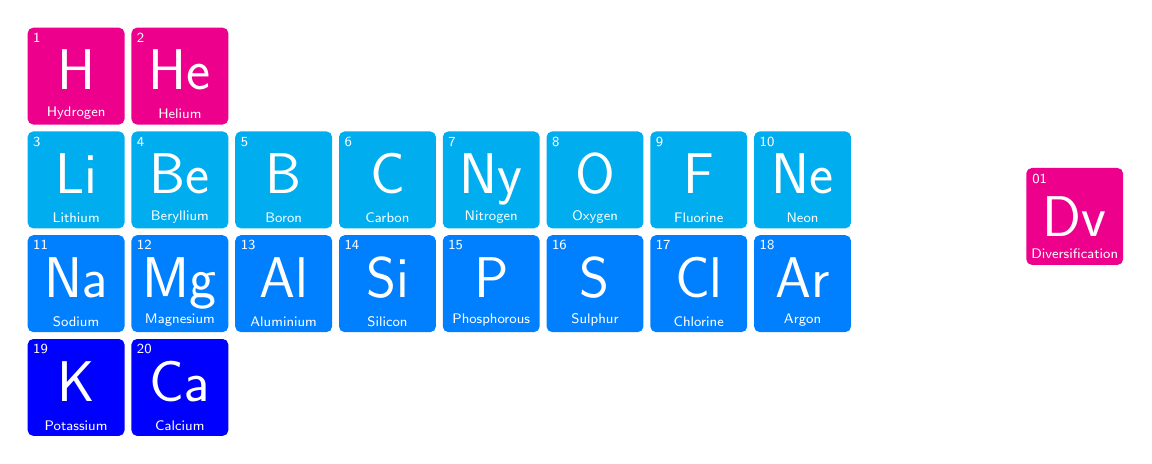
\begin{tikzpicture}[node distance=\elementsize]
\begin{scope}[xshift=0cm]
  \coordinate (o);
  \foreach \k/\m [count=\elementrow, evaluate=\elementrow as \elementshift using {-\elementrow*(\elementsize+\elementsep)}] in {%
    magenta/{H/Hydrogen,He/Helium},
    cyan/{%
      Li/Lithium,Be/Beryllium,B/Boron,C/Carbon,Ny/Nitrogen,
      O/Oxygen,F/Fluorine,Ne/Neon%
    },
    blue!50!cyan/{%
      Na/Sodium,Mg/Magnesium,Al/Aluminium,Si/Silicon,P/Phosphorous,
      S/Sulphur,Cl/Chlorine,Ar/Argon%
    },
    blue/{K/Potassium,Ca/Calcium}%
  }{%
    \coordinate (o\elementrow) at (0,\elementshift pt);
    \begin{scope}
      \foreach \i/\j [remember=\i as \ilast (initially o\elementrow)] in \m
      \pic [right=\elementsize+\elementsep of \ilast.mid] {element={name=\j, symbol=\i, fill=\k}};
    \end{scope}
  }
\end{scope}

\begin{scope}[xshift=14cm,yshift=-3cm]
    % Dv
    \coordinate (dv) at (0,0);
    \coordinate (base) at (35pt,0pt);
    \coordinate (height) at (0pt,35pt);
    \coordinate (diag) at ($(base)+(height)$);
    \fill[rounded corners=2pt, magenta] ($(dv)-.5*(diag)$) rectangle +(diag); 
    \node[white] at (dv) {\sffamily\huge Dv};
    \node[white, inner sep=2pt] (dvtext) at ($(dv)-.5*(height)$) [anchor=south] {\sffamily\tiny Diversification};
    \node[white, inner sep=2pt] (dvnum) at ($(dv)+.5*(height)-.5*(base)$) [anchor=north west] {\sffamily\tiny 01};
\end{scope}

\end{tikzpicture}
\end{document}
